% !TEX program = latexmk
\documentclass[b5paper,UTF8]{book}

% omega_0
% mu_s
% mu_z

\usepackage{ctex}
% plan
\usepackage{geometry}
    \geometry{top = 0.8 in}
    \geometry{bottom = 1 in}
    \geometry{left = 0.5 in}
    \geometry{right = 0.5 in}
\usepackage{fancyhdr}
    \pagestyle{fancy}
    \fancyhead{}
    \fancyhead[LO,RE]{{\arabic{chapter}}}
    \fancyhead[RO,LE]{\rightmark}
% Chinese title
\usepackage{titlesec}
\titleformat{\chapter}{\centering\Huge\bfseries}{第\,\thechapter\,章}{1em}{}
% formulas
\usepackage{amsmath}
% table
\usepackage{booktabs}
% pictures
\usepackage{graphicx}


% document
\begin{document}

% cover

\thispagestyle{empty}

\begin{center}
\vspace*{3 cm}

\heiti{\Huge{模板项目 \\ 计算书}}
\vspace*{1 cm}

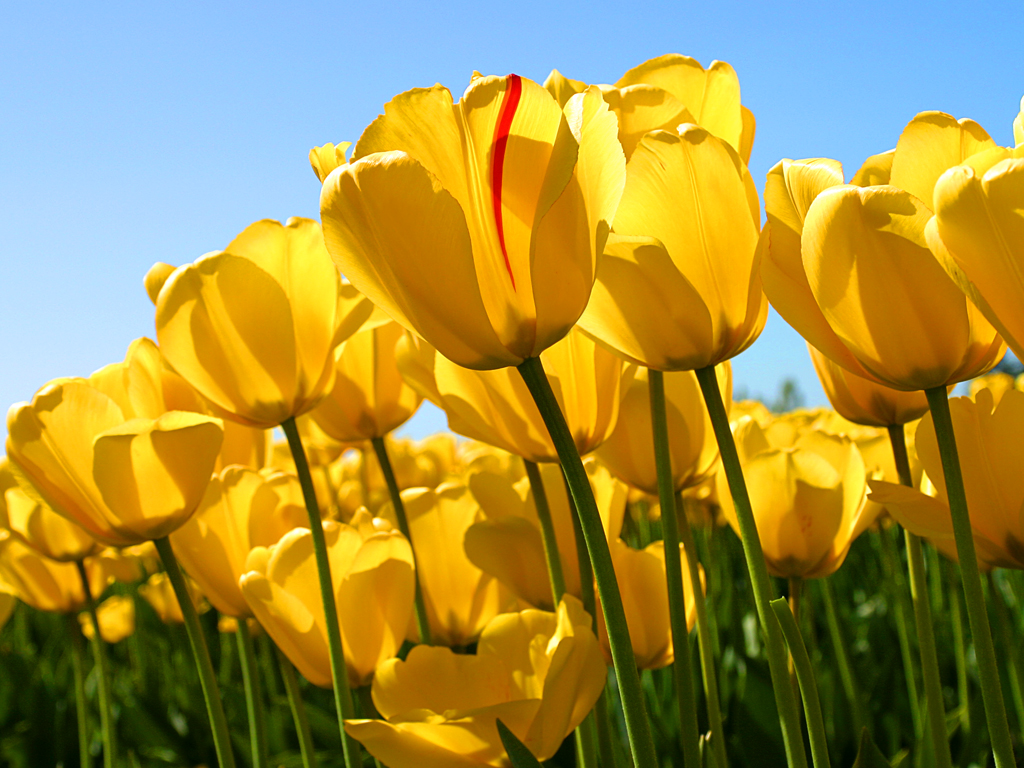
\includegraphics[width = 3 in]{cover.jpg}
\vspace*{1 cm}

\Large {2019 年 4 月 15 日}
\vspace*{0.5cm}

Will Clark
\end{center}
\vspace*{4cm}

\clearpage

% cover 2
\newpage
\thispagestyle{empty}

\noindent
书名: 《模板项目计算书》\\
作者: Will Clark\\
出版: 威尔出版社\\
版次: 2019 年 4 月 第 1 版\\
书号: ISBN 2-124-8765

\clearpage

% 目录
\setcounter{page}{1}
\pagenumbering{Roman}

\tableofcontents
% \thispagestyle{empty}

\clearpage


\setcounter{page}{1}
\pagenumbering{arabic}



\chapter{计算项目}

\section{已知条件}

已知参数:$a = #a$,$b = #b$。

\section{计算过程}

计算过程如下:

\begin{align*}
    c &= a + b \\
    &= #a + #b \\
    &= #c
\end{align*}


\section{计算结果}


求出结果:$c = #c$。

\end{document}
